\documentclass[letter,12pt]{article}
\usepackage[paperheight=27.94cm,paperwidth=21.59cm,bindingoffset=0in,left=3cm,right=2.0cm, top=3.5cm,bottom=2.5cm, headheight=200pt,headsep=1.0cm]{geometry}
\usepackage{graphicx,lastpage}
\usepackage{upgreek}
\usepackage{censor}
\usepackage[spanish,es-tabla]{babel}
\usepackage{pdfpages}
\usepackage{tabularx}
\usepackage{graphicx}
\usepackage{adjustbox}
\usepackage{xcolor}
\usepackage{colortbl}
\usepackage{rotating}
\usepackage{multirow}
\usepackage[utf8]{inputenc}
\usepackage{float}
\usepackage{hyperref}

\renewcommand{\tablename}{Tabla}
\usepackage{fancyhdr}
\pagestyle{fancy}

\usepackage{listing}
\usepackage{lstautogobble}
% Inline Code
\newcommand{\code}[1]{\colorbox{lightgray!80}{\lstinline[breaklines=true]|#1|}}
\newcommand{\BashCode}{
    \lstset{
        language=bash,
        basicstyle=\ttfamily\small,
        backgroundcolor=\color{lightgray!30},
        breaklines=true,
        showspaces=false,
        showstringspaces=false,
        numbers=left,
        % listings no tiene definido utf-8 por defecto
        % definimos cada carácter especial
        literate=
          {á}{{\'a}}1
          {é}{{\'e}}1
          {í}{{\'\i}}1
          {ó}{{\'o}}1
          {ú}{{\'u}}1
          {ñ}{{\~n}}1
          {¡}{{!`}}1
          {¿}{{?`}}1
      }
}
\definecolor{jpurple}{rgb}{0.5,0,0.35}
\newcommand{\RubyCode}{
    \lstset{
        language=ruby,
        basicstyle=\ttfamily\small,
        keywordstyle=\color{jpurple}\bfseries,
        stringstyle=\color{red},
        backgroundcolor=\color{lightgray!30},
        breaklines=true,
        showspaces=false,
        showstringspaces=false,
        numbers=left,
        % listings no tiene definido utf-8 por defecto
        % definimos cada carácter especial
        literate=
          {á}{{\'a}}1
          {é}{{\'e}}1
          {í}{{\'\i}}1
          {ó}{{\'o}}1
          {ú}{{\'u}}1
          {ñ}{{\~n}}1
          {¡}{{!`}}1
          {¿}{{?`}}1
      }
}

\begin{document}
   \title{\Huge{Informe Laboratorio 3}}
   \author{\textbf{Sección 3} \\  \\ Alan Toro\\ e-mail: alan.toro@mail.udp.cl}
   \date{Octubre de 2023}
   \maketitle
   \tableofcontents
  \newpage

\section{Descripción de actividades}
Su informante quiere entregarle la contraseña de acceso a una red, pero
desconfía de todo medio para entregársela (aún no llega al capítulo del curso en
donde aprende a comunicar una password sin que nadie más la pueda interceptar).
Por lo tanto, le entregará un archivo que contiene un desafío de autenticación,
que al analizarlo, usted podrá obtener la contraseña que lo permite resolver.
Como nadie puede ver a su informante (es informante y debe mantener el
anonimato), él se comunicará con usted a través de la redes inalámbricas y de
una forma que solo usted, como experto en informática y telecomunicaciones,
logrará esclarecer.

\begin{enumerate}
    \item Identifique cual es la red inalámbrica que está utilizando su
    informante para enviarle información. Obtenga la contraseña de esa red
    utilizando el ataque por defecto de aircrack-ng, indicando el tiempo requerido
    para esto. Descifre el contenido transmitido sobre ella y descargue de Internet
    el archivo que su informante le ha comunicado a través de los paquetes que usted
    ha descifrado.
    \item Descargue el diccionario de RockyouLinks to an external site.
    (utilizado ampliamente en el mundo del pentesting). Haga un script que para cada
    string contenido en el diccionario, reemplace la primera letra por su letra en
    capital y agregue un cero al final de la password.
    \item Todos los strings que comiencen con número toca eliminarlos del
    diccionario. Indique la cantidad de contraseñas que contiene el diccionario
    modificado debe llamarse rockyou\_mod.dic A continuación un ejemplo de cómo se
    modifican las 10 primeras líneas del diccionario original.
\end{enumerate}

\section{Desarrollo (PASO 1)}
La siguiente actividad será realizada usando un computador con Garuda Linux
(Linux-Zen 6.5.8) con una tarjeta de red integrada (Intel Cannon Point-LP CNVi).
Además, para la ejecución de esta se usa la tarjeta de red en modo monitor. Para
esto se utiliza el comando \code{sudo airmon check} para comprobar los servicios
que están haciendo uso de la tarjeta de red.

\begin{figure}[H]
  \centering
  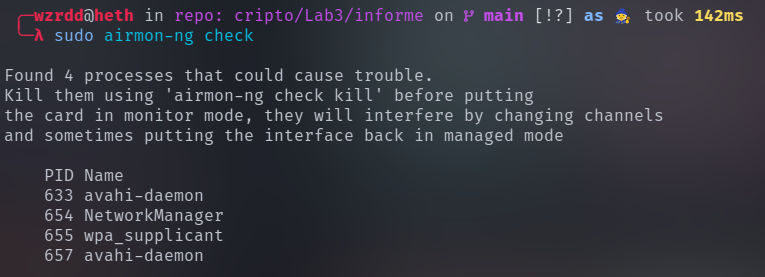
\includegraphics[width=16cm]{images/02-airmon-check.png}
  \caption{Procesos que podrían generar conflictos para iniciar el modo monitor.}
\end{figure}

Se usan 3 comandos para detener estos procesos.

\begin{listing}
    \BashCode{}
  \begin{lstlisting}
sudo systemctl stop wpa_supplicant
sudo systemctl stop NetworkManager
sudo systemctl disable --now avahi-daemon
  \end{lstlisting}
\end{listing}

Luego de esto, identificamos la tarjeta de red wifi a utilizar para todo el
laboratorio utilizando \code{iwconfig}, a lo que identificamos la interfaz
\textbf{wlp0s20f3} y bastaría con usar el comando \code{sudo airmon-ng start
wlp0s20f3} para colocar la tarjeta en modo monitor, esto cambia el nombre de la
interfaz a \textbf{wlp0s20f3mon}.

\begin{figure}[H]
  \centering
  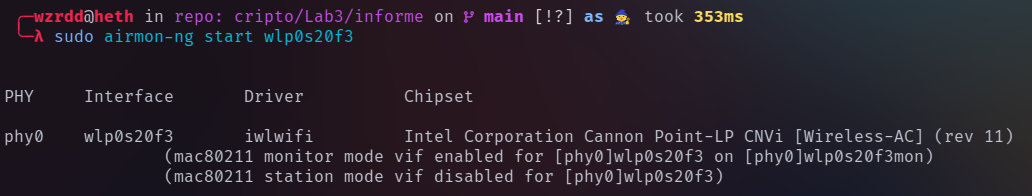
\includegraphics[width=16cm]{images/03-monitor-mode.png}
  \caption{Correcto cambio a modo monitor de la interfaz wlp0s20f3.}
\end{figure}

\subsection{Identificar en qué se destaca la red del informante del resto}
Para listar las redes disponibles, se usa el comando \code{nmcli dev wifi},
dentro de la lista de redes se nota una única red con cifrado WEP, protocolo
obsoleto, inseguro y atacable.

\subsection{Explica matemáticamente porqué se requieren más de 5000 paquetes para obtener la pass}
El ataque para obtener la pass es un ataque de colisión por fuerza bruta, en
particular un ataque de cumpleaños (\textit{Birthday Attack}), en este se dice
que la probailidad de encontrar paquete con un vector de inicialización
duplicado desde $\sqrt{n}$ donde n es la cantidad de vectores posibles comienza
a ser del 50\%.  Se sabe que el protocolo WEP utiliza vectores de inicialización
de 24 bits, por lo que n = $2^{24}$, lo que implica que desde
$\sqrt{2^{24}} = 4.096$ paquetes la probabilidad de encontrar un paquete
duplicado comienza a ser del 50\%. Es por esto que un buen número para comenzar
a romper la contraseña es del orden de los 5.000 vectores de inicialización.

\subsection{Obtiene la password con ataque por defecto de aircrack-ng}
Para obtener los IV, identificamos que la red WEP se encuentra en el canal 3 y
su bssid corresponde a B0:48:7A:D2:DD:74. Con esto podemos dirigir el ataque
directamente hacia la red víctima. Esto se realiza con el comando:

\begin{listing}
    \BashCode{}
  \begin{lstlisting}
sudo airodump-ng -c 3 --bssid B0:48:7A:D2:DD:74 -w dump wlp0s20f3mon
  \end{lstlisting}
\end{listing}

En donde la flag \code{-c 3} indica el canal y \code{-bssid B0:48:7A:D2:DD:74}
indican el canal de la víctima y la dirección física. El flag \code{-w dump}
genera un output en archivos dump.csv y dump.cap que serán utilizados por
\code{aircrack-ng} para obtener la pass. Finalmente se indica la interfaz de red
\textbf{wlp0s20f3mon}.

\begin{figure}[H]
  \centering
  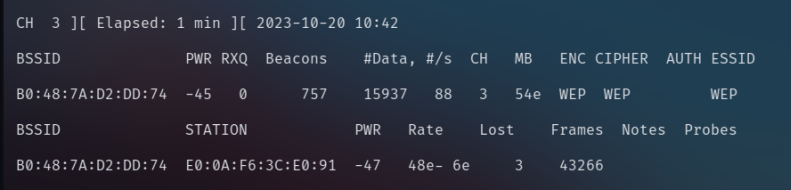
\includegraphics[width=16cm]{images/04-output-airodump.png}
  \caption{Comando airodump dirigido hacia la víctima capturando IVs.}
\end{figure}

Se logra obtener la contraseña con más de 20.000 IVs. En particular con 23.034 IVs.
El comando airodump anteriormente descrito genera un archivo dump-01.cap, este archivo se usa como entrada para ejecutar el comando:

\begin{listing}
    \BashCode{}
  \begin{lstlisting}
sudo aircrack-ng -b B0:48:7A:D2:DD:74 dump-01.cap
  \end{lstlisting}
\end{listing}

Este comando cada 5.000 IVs intenta crackear la pass. Finalmente en los 23.034 se logra esto:

\begin{figure}[H]
  \centering
  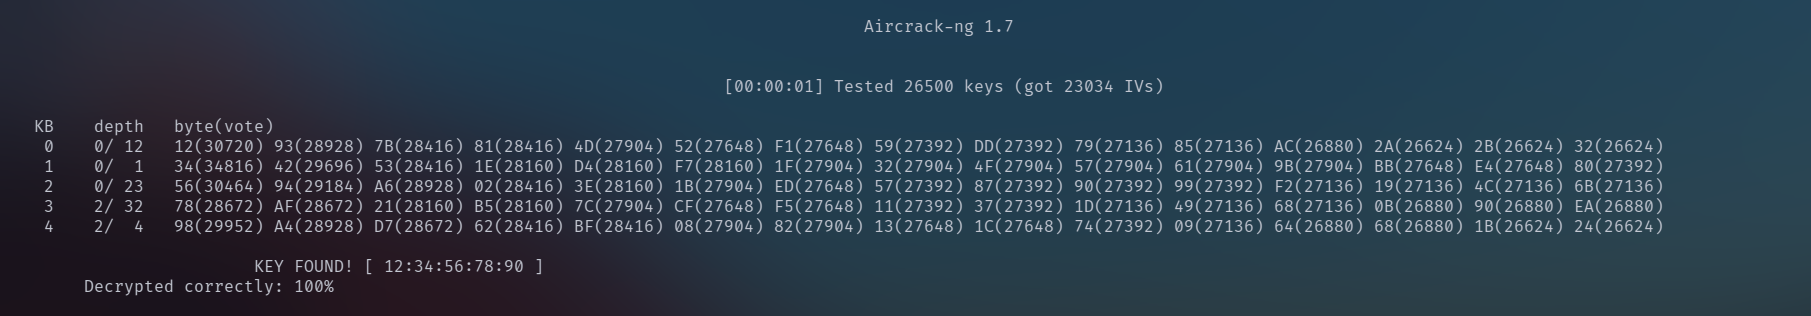
\includegraphics[width=16cm]{images/05-decrypted.png}
  \caption{Comando aircrack-ng con la contraseña encontrada.}
\end{figure}

La contraseña de la red es \code{12:34:56:78:90}.

\subsection{Indica el tiempo que demoró en obtener la password}
El tiempo de captura total fue de 2 minutos y 7 segundos. Esto se puede
verificar en el archivo dump-01.csv entonce la hora de inicio de captura fue en
2023-10-20 10:40:50 y el tiempo de término fue 2023-10-20 10:42:57. Además, con
los IVs ya capturados crackear la contraseña tomó 1 segundo, esto se puede ver
en la figura 4 de la subsección anterior.

\subsection{Descifra el contenido capturado}
Para decifrar el tráfico se utiliza el comando \code{sudo airdecap-ng -w
12:34:56:78:90 dump-01.cap} en donde la flag \code{-w 12:34:56:78:90}
corresponde a la contraseña encontrada y dump-01.cap al archivo de la captura de
airodump de la sección anterior. El resultado de este comando es la generación
del  archivo \textbf{dump-01-dec.cap}.

\begin{figure}[H]
  \centering
  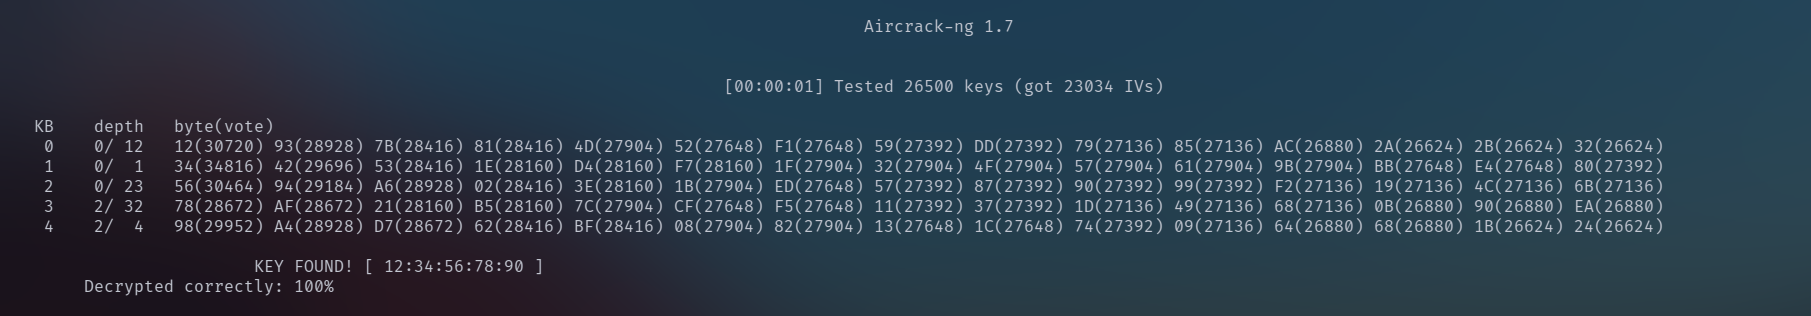
\includegraphics[width=16cm]{images/05-decrypted.png}
  \caption{Comando airedecap decifrando los paquetes.}
\end{figure}

\subsection{Describe como obtiene la url de donde descargar el archivo}
Finalmente, se analizan los paquetes capturados usando Wireshark. A inspección
simple se encuentra un flujo constante de paquetes ICMP, en donde, todos en el
payload tienen una URL.

\begin{figure}[H]
  \centering
  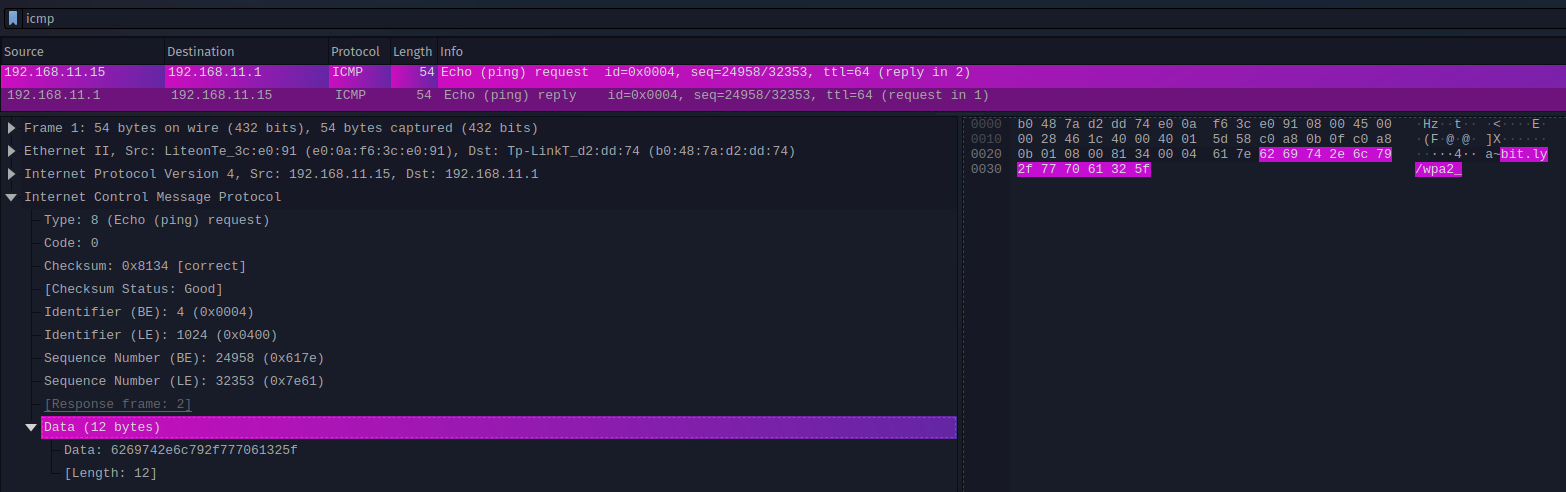
\includegraphics[width=16cm]{images/06-wireshark.png}
  \caption{Payload de un paquete ICMP capturado en donde se encuentra la URL.}
\end{figure}

La URL redirige hacia \url{https://www.cloudshark.org/captures/b5b39e1c51eb} en
donde se encuentra la captura de un handshake.

\section{Desarrollo (PASO 2)}
\subsection{Indica script para modificar diccionario original}
Para generar un diccionario modificado se usa un script escrito en Ruby. Adjunto en el proyecto como \code{codigos/modify_dict.rb} que también se muestra a continuación:

\begin{listing}
    \RubyCode{}
  \begin{lstlisting}
File.open("rockyou.txt", :encoding => 'iso-8859-15') do |input_file|
  File.open("rockyou_mod.dic", "w") do |output_file|
    input_file.each_line do |line|
      if !line.match?(/\A\d/)
        output_file.puts line.capitalize.strip + '0'
      end
    end
  end
end
  \end{lstlisting}
\end{listing}

Lo que genera un nuevo diccionario llamado \textbf{rockyou\_mod.dic}.

\subsection{Cantidad de passwords finales que contiene rockyou\_mod.dic}
Cada contraseña es una columna por lo que se cuentan la cantidad de filas del archivo generado usando \code{wc -l}. Lo indica 11.059.798 de contraseñas finales.

\begin{figure}[H]
  \centering
  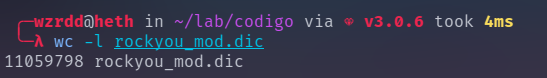
\includegraphics[width=16cm]{images/07-lines-mod-dic.png}
  \caption{Cantidad de passwors finales.}
\end{figure}

\section{Desarrollo (Paso 3)}
Con el archivo encontrado en el paso uso \textbf{handshake.pcap} conventimos a
formato hc22000 para recuperar una PSK. Para esto usamos el comando:

\begin{listing}
    \BashCode{}
  \begin{lstlisting}
hcxpcapngtool -o handshake.hc22000 handshake.pcapng
  \end{lstlisting}
\end{listing}

\subsection{Obtiene contraseña con hashcat con potfile}
Para obtener la contraseña usando hashcat se usa el comando:

\begin{listing}
    \BashCode{}
  \begin{lstlisting}
hashcat --potfile-path potfile.txt -m 22000 handshake.hc22000 rockyou_mod.dic
  \end{lstlisting}
\end{listing}

Lo que genera el output:

\begin{figure}[H]
  \centering
  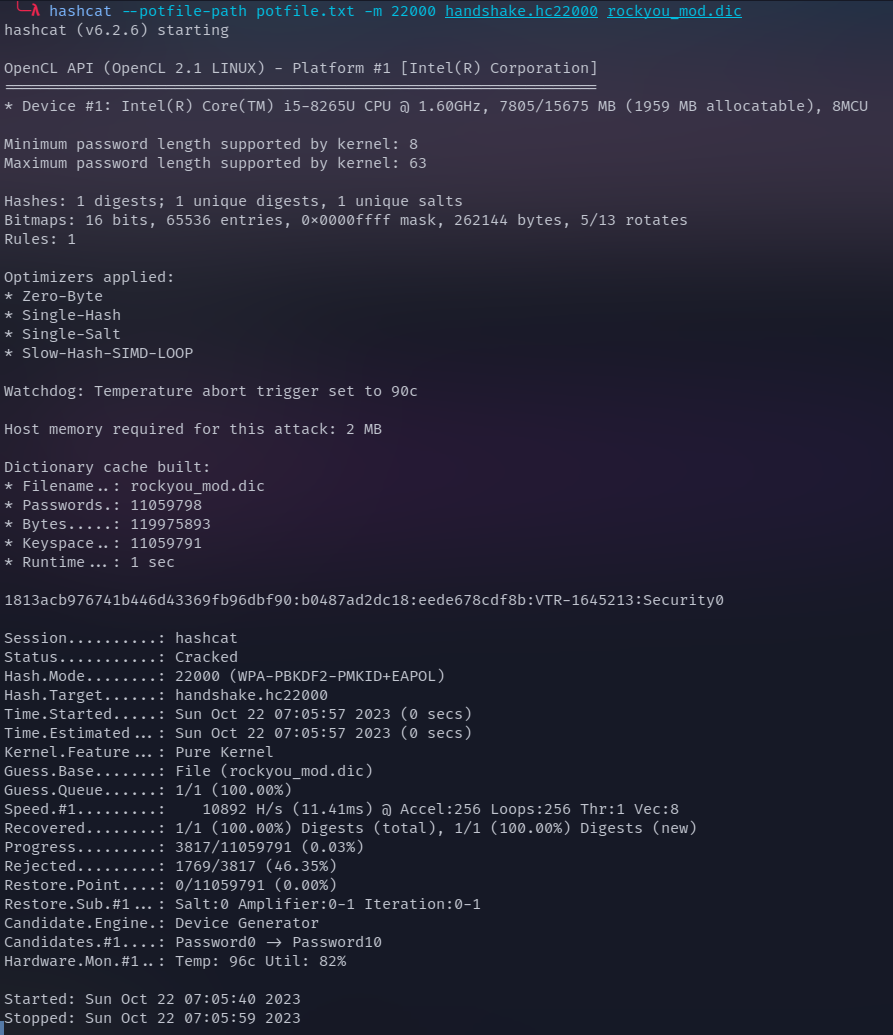
\includegraphics[width=16cm]{images/08-hashcat-with-potfile.png}
  \caption{Output hashcat con potfile.}
\end{figure}

La contraseña es SECURITY0 y el SSID es VTR-1645213, ambos se encuentran también en el potfile.

\subsection{Identifica nomenclatura del output}
\begin{itemize}
  \item Device: Describe la unidad de procesamiento encargada de ejecutar la fuerza bruta. En este caso fue una CPU integrada Intel i5-8265U.
  \item Se describe el mínimo y máximo largo que se puede procesar por el kernel. En este caso 8 mínimo y 63 máximo.
  \item Se detalla la cantidad de hashes y describen los bitmaps.
  \item Se indica la lista de optimizadores utilizados.
  \item Watchdog determina una temperatura máxima del device, si se supera se aborta la tarea.
  \item Se describe el cache del diccionario.
  \item Se listan los hash y credenciales \textit{crackeados}.
  \item Entre los más importantes que siguen está: el estado como crackeado, el modo de hash, los tiempos de inicio y término, la velocidad de hasheado y los candidatos siguientes.
\end{itemize}

\subsection{Obtiene contraseña con hashcat sin potfile}
Para obtener la contraseña usando hashcat sin potfile se usa la flag
\code{--potfile-disable}. El comando a usar queda como:

\begin{listing}
    \BashCode{}
  \begin{lstlisting}
hashcat --potfile-disable -m 22000 handshake.hc22000 rockyou_mod.dic
  \end{lstlisting}
\end{listing}

Lo que genera el output:

\begin{figure}[H]
  \centering
  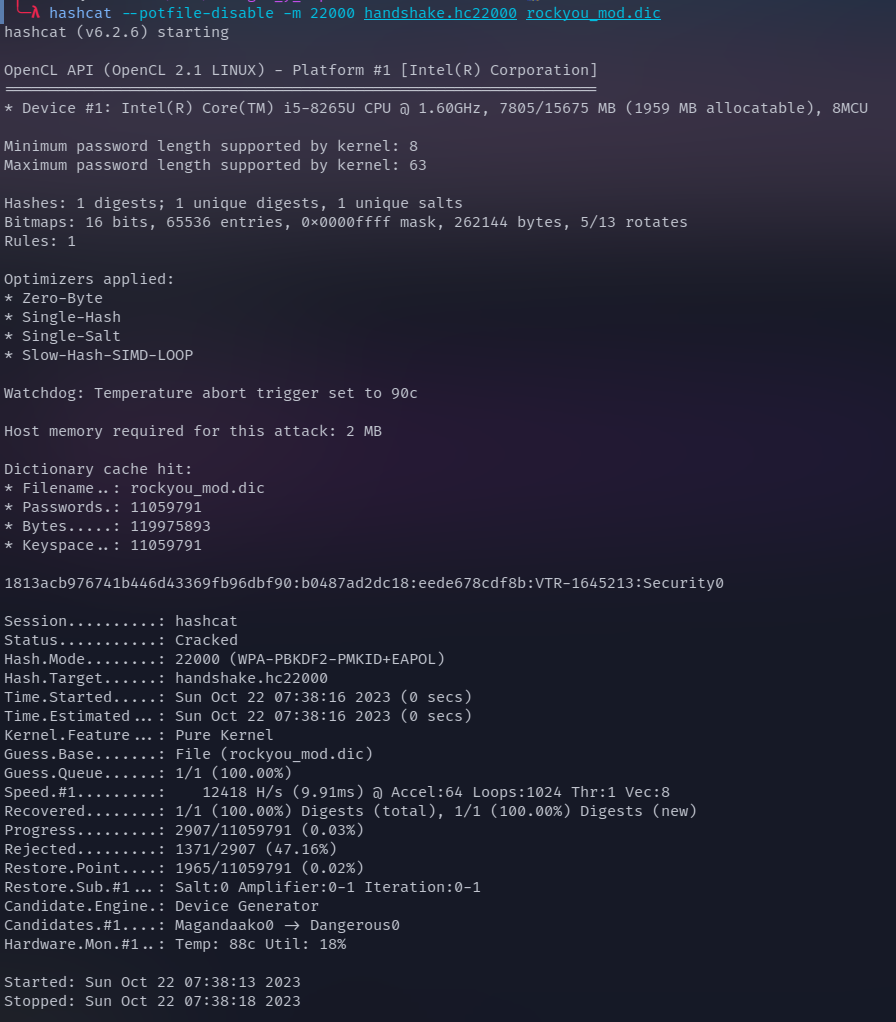
\includegraphics[width=16cm]{images/09-hashcat-potfile-disable.png}
  \caption{Output hashcat sin potfile.}
\end{figure}

Se llega a la misma contraseña y SSID que la sección anterior con potfile.

\subsection{Identifica nomenclatura del output}

\begin{itemize}
  \item Device: Describe la unidad de procesamiento encargada de ejecutar la fuerza bruta. En este caso fue una CPU integrada Intel i5-8265U.
  \item Se describe el mínimo y máximo largo que se puede procesar por el kernel. En este caso 8 mínimo y 63 máximo.
  \item Se detalla la cantidad de hashes y describen los bitmaps.
  \item Se indica la lista de optimizadores utilizados.
  \item Watchdog determina una temperatura máxima del device, si se supera se aborta la tarea.
  \item Se describe el cache del diccionario.
  \item Se listan los hash y credenciales \textit{crackeados}.
  \item Entre los más importantes que siguen está: el estado como crackeado, el modo de hash, los tiempos de inicio y término, la velocidad de hasheado y los candidatos siguientes.
\end{itemize}

\subsection{Obtiene contraseña con aircrack-ng}
Para encontrar la contraseña usando aircrack-ng se usa el comando:

\begin{listing}
    \BashCode{}
  \begin{lstlisting}
aircrack-ng -w rockyou_mod.dic handshake.pcap
  \end{lstlisting}
\end{listing}

Lo que genera el output

\begin{figure}[H]
  \centering
  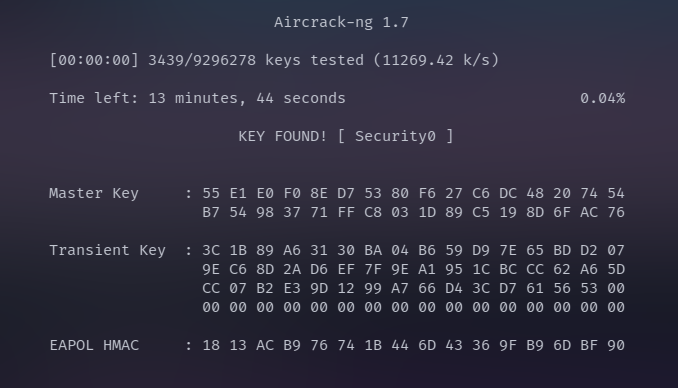
\includegraphics[width=16cm]{images/10-aircrack-founded.png}
  \caption{Output aircrack encontrando la contraseña.}
\end{figure}

También converge a la contraseña SECURITY0.

\subsection{Identifica y modifica parámetros solicitados por pycrack}
Los parámetros a modificar son:

\begin{itemize}
  \item Path del archivo al diccionario.
  \item El SSID que se puede encontrar en el primer paquete o desde el output de hashcat de la sección anterior.
  \item El Authenticator y Supplicant Nounce. Estos se pueden encontrar en el primer y segundo mensaje del protocolo EAPOL respectivamente. En el apartado ``802.1X Authentication'', en el campo ``WPA Key Nonce'' de cada uno.
  \item  Las direcciones físicas del Authenticator y Supplicant, se puede encontrar en todos los paquetes EAPOL.
  \item  El MIC1 se encuentra en el segundo paquete del protocolo EAPOL, el MIC2 en el tercer paquete EAPOL y el MIC se encuentra en el cuarto paquete.
  \item Los campos DATA1, 2 y 3 son el bloque completo de ``802.1X Authentication'' como hexadecimal.
\end{itemize}

Todos los cambios están comentados al final de la línea como un ``CAMBIADO'' para identificarlos en el código pywd.py adjunto en el proyecto.

\subsection{Obtiene contraseña con pycrack}

\begin{figure}[H]
  \centering
  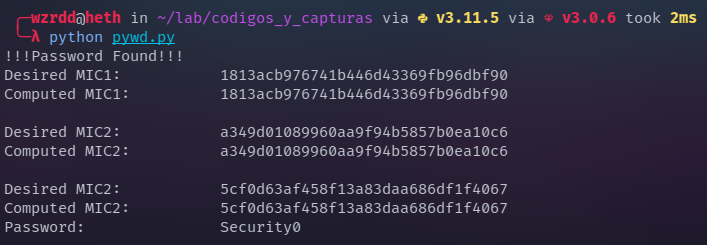
\includegraphics[width=16cm]{images/11-pycrack-founded.png}
  \caption{Output pycrack encontrando la contraseña}
\end{figure}

Al igual que los otros métodos, encuentra la contraseña SECURITY0.

\section*{Conclusiones y comentarios}
Primero que todo, la conclusión más importante es el poco tiempo que tomó quebrar todas las seguridades. En el caso de WEP se logró enocntrar una contraseña segura de largo 15 en un tiempo aproximado de 2 minutos. Esto quiere decir que contraseñas seguras sobre protocolos inseguros no mejoran la seguridad ya que la seguridad se pierde por el hilo más fino. En este caso particular un ataque de colisiones por fuerza bruta es suficiente para exponer la red.

Con respecto a los siguientes pasos los tiempos también fueron extremadamente cortos en un computador de recursos medios. Es por esto que para auditar la seguridad de una red valga la pena revisar diccionarios comunes y variantes que se pueden lograr a partir de estos. Ya que, un ataque por diccionario a un tráfico interceptado puede exponer la red de manera rápida y fácil incluso utilizando protocolos seguros como WPA.

\section*{Enlace a Github}
- \url{https://github.com/wzrdd/cripto}
\end{document}
